%\input{Preambulum}

\begin{figure}[t!]
\centering
\begin{subfigure}{0.24\textwidth}
\centering
\caption{$I_1$: $7$ excl., \#4238}
% (2017 reversed)
\label{Fig3a}

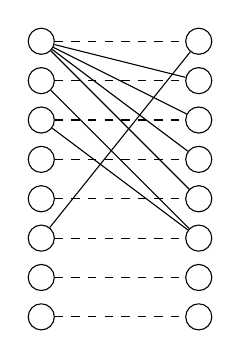
\begin{tikzpicture}[scale=1, auto=center]
\tikzstyle{every node}=[draw,shape=circle];
  \node[minimum size=0.25cm] (n1) at (0,3.5) {};
  \node[minimum size=0.25cm] (n2) at (0,3)   {};
  \node[minimum size=0.25cm] (n3) at (0,2.5) {};
  \node[minimum size=0.25cm] (n4) at (0,2)   {};
  \node[minimum size=0.25cm] (n5) at (0,1.5) {};
  \node[minimum size=0.25cm] (n6) at (0,1)   {};
  \node[minimum size=0.25cm] (n7) at (0,0.5) {};
  \node[minimum size=0.25cm] (n8) at (0,0)   {};
  \node[minimum size=0.25cm] (n9) at (2,3.5) {};
  \node[minimum size=0.25cm] (n10) at (2,3)   {};
  \node[minimum size=0.25cm] (n11) at (2,2.5) {};
  \node[minimum size=0.25cm] (n12) at (2,2)   {};
  \node[minimum size=0.25cm] (n13) at (2,1.5) {};
  \node[minimum size=0.25cm] (n14) at (2,1)   {};
  \node[minimum size=0.25cm] (n15) at (2,0.5) {};
  \node[minimum size=0.25cm] (n16) at (2,0)   {};

  \foreach \from/\to in {n1/n9,n2/n10,n3/n11,n4/n12,n5/n13,n6/n14,n7/n15,n8/n16}
    \draw[dashed] (\from) -- (\to);
  \foreach \from/\to in {n1/n10,n1/n11,n1/n12,n1/n13,n2/n14,n3/n14,n6/n9}
    \draw (\from) -- (\to);
\end{tikzpicture}
\end{subfigure}
\begin{subfigure}{0.24\textwidth}
\centering
\caption{$I_2$: $8$ excl., \#3620}
\label{Fig3b}

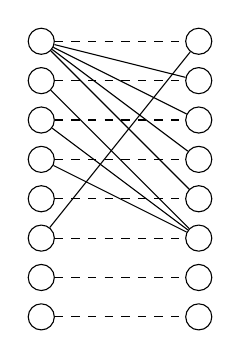
\begin{tikzpicture}[scale=1, auto=center]
\tikzstyle{every node}=[draw,shape=circle];
  \node[minimum size=0.25cm] (n1) at (0,3.5) {};
  \node[minimum size=0.25cm] (n2) at (0,3)   {};
  \node[minimum size=0.25cm] (n3) at (0,2.5) {};
  \node[minimum size=0.25cm] (n4) at (0,2)   {};
  \node[minimum size=0.25cm] (n5) at (0,1.5) {};
  \node[minimum size=0.25cm] (n6) at (0,1)   {};
  \node[minimum size=0.25cm] (n7) at (0,0.5) {};
  \node[minimum size=0.25cm] (n8) at (0,0)   {};
  \node[minimum size=0.25cm] (n9) at (2,3.5) {};
  \node[minimum size=0.25cm] (n10) at (2,3)   {};
  \node[minimum size=0.25cm] (n11) at (2,2.5) {};
  \node[minimum size=0.25cm] (n12) at (2,2)   {};
  \node[minimum size=0.25cm] (n13) at (2,1.5) {};
  \node[minimum size=0.25cm] (n14) at (2,1)   {};
  \node[minimum size=0.25cm] (n15) at (2,0.5) {};
  \node[minimum size=0.25cm] (n16) at (2,0)   {};

  \foreach \from/\to in {n1/n9,n2/n10,n3/n11,n4/n12,n5/n13,n6/n14,n7/n15,n8/n16}
    \draw[dashed] (\from) -- (\to);
  \foreach \from/\to in {n1/n10,n1/n11,n1/n12,n1/n13,n2/n14,n3/n14,n4/n14,n6/n9}
    \draw (\from) -- (\to);
\end{tikzpicture}
\end{subfigure}
\begin{subfigure}{0.24\textwidth}
\centering
\caption{$I_3$: $8$ excl., 3854}
\label{Fig3c}

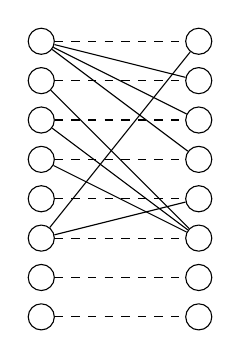
\begin{tikzpicture}[scale=1, auto=center]
\tikzstyle{every node}=[draw,shape=circle];
  \node[minimum size=0.25cm] (n1) at (0,3.5) {};
  \node[minimum size=0.25cm] (n2) at (0,3)   {};
  \node[minimum size=0.25cm] (n3) at (0,2.5) {};
  \node[minimum size=0.25cm] (n4) at (0,2)   {};
  \node[minimum size=0.25cm] (n5) at (0,1.5) {};
  \node[minimum size=0.25cm] (n6) at (0,1)   {};
  \node[minimum size=0.25cm] (n7) at (0,0.5) {};
  \node[minimum size=0.25cm] (n8) at (0,0)   {};
  \node[minimum size=0.25cm] (n9) at (2,3.5) {};
  \node[minimum size=0.25cm] (n10) at (2,3)   {};
  \node[minimum size=0.25cm] (n11) at (2,2.5) {};
  \node[minimum size=0.25cm] (n12) at (2,2)   {};
  \node[minimum size=0.25cm] (n13) at (2,1.5) {};
  \node[minimum size=0.25cm] (n14) at (2,1)   {};
  \node[minimum size=0.25cm] (n15) at (2,0.5) {};
  \node[minimum size=0.25cm] (n16) at (2,0)   {};

  \foreach \from/\to in {n1/n9,n2/n10,n3/n11,n4/n12,n5/n13,n6/n14,n7/n15,n8/n16}
    \draw[dashed] (\from) -- (\to);
  \foreach \from/\to in {n1/n10,n1/n11,n1/n12,n2/n14,n3/n14,n4/n14,n6/n9,n6/n13}
    \draw (\from) -- (\to);
\end{tikzpicture}
\end{subfigure}
\begin{subfigure}{0.24\textwidth}
\centering
\caption{$I_4$: $9$ excl., \#3002}
\label{Fig3d}

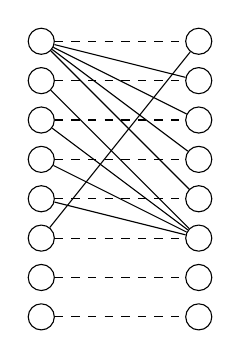
\begin{tikzpicture}[scale=1, auto=center]
\tikzstyle{every node}=[draw,shape=circle];
  \node[minimum size=0.25cm] (n1) at (0,3.5) {};
  \node[minimum size=0.25cm] (n2) at (0,3)   {};
  \node[minimum size=0.25cm] (n3) at (0,2.5) {};
  \node[minimum size=0.25cm] (n4) at (0,2)   {};
  \node[minimum size=0.25cm] (n5) at (0,1.5) {};
  \node[minimum size=0.25cm] (n6) at (0,1)   {};
  \node[minimum size=0.25cm] (n7) at (0,0.5) {};
  \node[minimum size=0.25cm] (n8) at (0,0)   {};
  \node[minimum size=0.25cm] (n9) at (2,3.5) {};
  \node[minimum size=0.25cm] (n10) at (2,3)   {};
  \node[minimum size=0.25cm] (n11) at (2,2.5) {};
  \node[minimum size=0.25cm] (n12) at (2,2)   {};
  \node[minimum size=0.25cm] (n13) at (2,1.5) {};
  \node[minimum size=0.25cm] (n14) at (2,1)   {};
  \node[minimum size=0.25cm] (n15) at (2,0.5) {};
  \node[minimum size=0.25cm] (n16) at (2,0)   {};

  \foreach \from/\to in {n1/n9,n2/n10,n3/n11,n4/n12,n5/n13,n6/n14,n7/n15,n8/n16}
    \draw[dashed] (\from) -- (\to);
  \foreach \from/\to in {n1/n10,n1/n11,n1/n12,n1/n13,n2/n14,n3/n14,n4/n14,n5/n14,n6/n9}
    \draw (\from) -- (\to);
\end{tikzpicture}
\end{subfigure}

\vspace{0.25cm}
\begin{subfigure}{0.24\textwidth}
\centering
\caption{$I_5$: $9$ excl., \#3077}
\label{Fig3e}

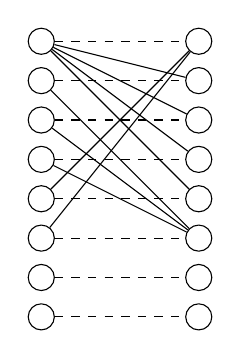
\begin{tikzpicture}[scale=1, auto=center]
\tikzstyle{every node}=[draw,shape=circle];
  \node[minimum size=0.25cm] (n1) at (0,3.5) {};
  \node[minimum size=0.25cm] (n2) at (0,3)   {};
  \node[minimum size=0.25cm] (n3) at (0,2.5) {};
  \node[minimum size=0.25cm] (n4) at (0,2)   {};
  \node[minimum size=0.25cm] (n5) at (0,1.5) {};
  \node[minimum size=0.25cm] (n6) at (0,1)   {};
  \node[minimum size=0.25cm] (n7) at (0,0.5) {};
  \node[minimum size=0.25cm] (n8) at (0,0)   {};
  \node[minimum size=0.25cm] (n9) at (2,3.5) {};
  \node[minimum size=0.25cm] (n10) at (2,3)   {};
  \node[minimum size=0.25cm] (n11) at (2,2.5) {};
  \node[minimum size=0.25cm] (n12) at (2,2)   {};
  \node[minimum size=0.25cm] (n13) at (2,1.5) {};
  \node[minimum size=0.25cm] (n14) at (2,1)   {};
  \node[minimum size=0.25cm] (n15) at (2,0.5) {};
  \node[minimum size=0.25cm] (n16) at (2,0)   {};

  \foreach \from/\to in {n1/n9,n2/n10,n3/n11,n4/n12,n5/n13,n6/n14,n7/n15,n8/n16}
    \draw[dashed] (\from) -- (\to);
  \foreach \from/\to in {n1/n10,n1/n11,n1/n12,n1/n13,n2/n14,n3/n14,n4/n14,n5/n9,n6/n9}
    \draw (\from) -- (\to);
\end{tikzpicture}
\end{subfigure}
\begin{subfigure}{0.24\textwidth}
\centering
\caption{$I_6$: $9$ excl., \#2896}
\label{Fig3f}

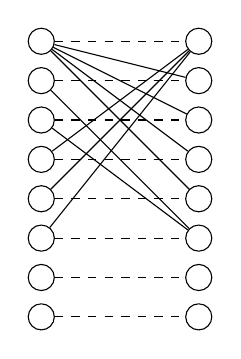
\begin{tikzpicture}[scale=1, auto=center]
\tikzstyle{every node}=[draw,shape=circle];
  \node[minimum size=0.25cm] (n1) at (0,3.5) {};
  \node[minimum size=0.25cm] (n2) at (0,3)   {};
  \node[minimum size=0.25cm] (n3) at (0,2.5) {};
  \node[minimum size=0.25cm] (n4) at (0,2)   {};
  \node[minimum size=0.25cm] (n5) at (0,1.5) {};
  \node[minimum size=0.25cm] (n6) at (0,1)   {};
  \node[minimum size=0.25cm] (n7) at (0,0.5) {};
  \node[minimum size=0.25cm] (n8) at (0,0)   {};
  \node[minimum size=0.25cm] (n9) at (2,3.5) {};
  \node[minimum size=0.25cm] (n10) at (2,3)   {};
  \node[minimum size=0.25cm] (n11) at (2,2.5) {};
  \node[minimum size=0.25cm] (n12) at (2,2)   {};
  \node[minimum size=0.25cm] (n13) at (2,1.5) {};
  \node[minimum size=0.25cm] (n14) at (2,1)   {};
  \node[minimum size=0.25cm] (n15) at (2,0.5) {};
  \node[minimum size=0.25cm] (n16) at (2,0)   {};

  \foreach \from/\to in {n1/n9,n2/n10,n3/n11,n4/n12,n5/n13,n6/n14,n7/n15,n8/n16}
    \draw[dashed] (\from) -- (\to);
  \foreach \from/\to in {n1/n10,n1/n11,n1/n12,n1/n13,n2/n14,n3/n14,n4/n9,n5/n9,n6/n9}
    \draw (\from) -- (\to);
\end{tikzpicture}
\end{subfigure}
\begin{subfigure}{0.24\textwidth}
\centering
\caption{$I_7$: $8$ excl., \#3779}
\label{Fig3g}

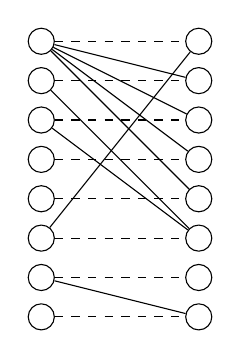
\begin{tikzpicture}[scale=1, auto=center]
\tikzstyle{every node}=[draw,shape=circle];
  \node[minimum size=0.25cm] (n1) at (0,3.5) {};
  \node[minimum size=0.25cm] (n2) at (0,3)   {};
  \node[minimum size=0.25cm] (n3) at (0,2.5) {};
  \node[minimum size=0.25cm] (n4) at (0,2)   {};
  \node[minimum size=0.25cm] (n5) at (0,1.5) {};
  \node[minimum size=0.25cm] (n6) at (0,1)   {};
  \node[minimum size=0.25cm] (n7) at (0,0.5) {};
  \node[minimum size=0.25cm] (n8) at (0,0)   {};
  \node[minimum size=0.25cm] (n9) at (2,3.5) {};
  \node[minimum size=0.25cm] (n10) at (2,3)   {};
  \node[minimum size=0.25cm] (n11) at (2,2.5) {};
  \node[minimum size=0.25cm] (n12) at (2,2)   {};
  \node[minimum size=0.25cm] (n13) at (2,1.5) {};
  \node[minimum size=0.25cm] (n14) at (2,1)   {};
  \node[minimum size=0.25cm] (n15) at (2,0.5) {};
  \node[minimum size=0.25cm] (n16) at (2,0)   {};

  \foreach \from/\to in {n1/n9,n2/n10,n3/n11,n4/n12,n5/n13,n6/n14,n7/n15,n8/n16}
    \draw[dashed] (\from) -- (\to);
  \foreach \from/\to in {n1/n10,n1/n11,n1/n12,n1/n13,n2/n14,n3/n14,n6/n9,n7/n16}
    \draw (\from) -- (\to);
\end{tikzpicture}
\end{subfigure}
\begin{subfigure}{0.24\textwidth}
\centering
\caption{$I_8$: $9$ excl., \#3152}
\label{Fig3h}

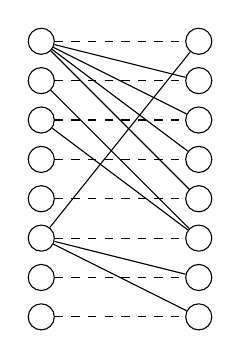
\begin{tikzpicture}[scale=1, auto=center]
\tikzstyle{every node}=[draw,shape=circle];
  \node[minimum size=0.25cm] (n1) at (0,3.5) {};
  \node[minimum size=0.25cm] (n2) at (0,3)   {};
  \node[minimum size=0.25cm] (n3) at (0,2.5) {};
  \node[minimum size=0.25cm] (n4) at (0,2)   {};
  \node[minimum size=0.25cm] (n5) at (0,1.5) {};
  \node[minimum size=0.25cm] (n6) at (0,1)   {};
  \node[minimum size=0.25cm] (n7) at (0,0.5) {};
  \node[minimum size=0.25cm] (n8) at (0,0)   {};
  \node[minimum size=0.25cm] (n9) at (2,3.5) {};
  \node[minimum size=0.25cm] (n10) at (2,3)   {};
  \node[minimum size=0.25cm] (n11) at (2,2.5) {};
  \node[minimum size=0.25cm] (n12) at (2,2)   {};
  \node[minimum size=0.25cm] (n13) at (2,1.5) {};
  \node[minimum size=0.25cm] (n14) at (2,1)   {};
  \node[minimum size=0.25cm] (n15) at (2,0.5) {};
  \node[minimum size=0.25cm] (n16) at (2,0)   {};

  \foreach \from/\to in {n1/n9,n2/n10,n3/n11,n4/n12,n5/n13,n6/n14,n7/n15,n8/n16}
    \draw[dashed] (\from) -- (\to);
  \foreach \from/\to in {n1/n10,n1/n11,n1/n12,n1/n13,n2/n14,n3/n14,n6/n9,n6/n15,n6/n16}
    \draw (\from) -- (\to);
\end{tikzpicture}
\end{subfigure}

\captionsetup{justification=centerfirst}
\caption{Some balanced bipartite graphs with 16 nodes \\ \vspace{0.2cm}
\footnotesize{\emph{Notes}: Dashed lines indicate the pair constraints, solid lines indicate the type constraints. \\
The number after \# shows the number of valid assignments.}}
\label{Fig3}
\end{figure}

%\end{document}